% !TeX root = Protokoll.tex
\subsection[Intensitätverteilung der $\mathrm{TEM_{00}}$]{Intensitätverteilung der $\mathbf{TEM_{00}}$}\label{sec:TEM00}
	Für die Bestimmung der Intensitätsverteilung in Abhängigkeit des Abstands zur optischen
	Achse wurde der Strom an der Photodiode in dieser Abhängigkeit aufgenommen.
	Dies so erhaltenen Messwerte sind in der \cref{tab:TEM00} eingetragen.
	\begin{table}[!h]
	\centering
	\begin{adjustbox}{width=1\textwidth}
	\begin{tabular}{cccccccc}
		\toprule
		Abstand & Photostrom & Abstand & Photostrom & Abstand & Photostrom & Abstand & Photostrom\\
		$r$/\si{mm} & $I$/\si{\micro\ampere} & $x$/\si{mm} & $I$/\si{\micro\ampere} & $r$/\si{mm} & $I$/\si{\micro\ampere} & $x$/\si{mm} & $I$/\si{\micro\ampere}\\
\midrule
		\num{-9(1)} & \num{14.2(1)} & \num{-1(1)} & \num{31.5(1)} & \num{7(1)} & \num{20.2(1)} & \num{15(1)} & \num{3.4(1)}\\
		\num{-8(1)} & \num{19.0(1)} & \num{0(1)} & \num{32.7(1)} & \num{8(1)} & \num{17.4(1)} & \num{16(1)} & \num{2.9(1)}\\
		\num{-7(1)} & \num{20.0(1)} & \num{1(1)} & \num{29.2(1)} & \num{9(1)} & \num{14.4(1)} & \num{17(1)} & \num{2.4(1)}\\
		\num{-6(1)} & \num{21.1(1)} & \num{2(1)} & \num{29.5(1)} & \num{10(1)} & \num{12.4(1)} & \num{18(1)} & \num{1.3(1)}\\
		\num{-5(1)} & \num{24.0(1)} & \num{3(1)} & \num{28.1(1)} & \num{11(1)} & \num{9.6(1)} & \num{19(1)} & \num{0.9(1)}\\
		\num{-4(1)} & \num{27.1(1)} & \num{4(1)} & \num{28.6(1)} & \num{12(1)} & \num{7.2(1)} & \num{20(1)} & \num{0.7(1)}\\
		\num{-3(1)} & \num{28.8(1)} & \num{5(1)} & \num{27.1(1)} & \num{13(1)} & \num{6.2(1)} & \num{21(1)} & \num{0.5(1)}\\
		\num{-2(1)} & \num{31.7(1)} & \num{6(1)} & \num{25.4(1)} & \num{14(1)} & \num{4.3(1)} & \num{22(1)} & \num{0.4(1)}\\
		\bottomrule
	\end{tabular}
	\end{adjustbox}
	\caption{Messwerte des Photostroms in Abhaengigkeit des Abstands zur optischen Achse. \label{tab:TEM00}}
	
\end{table}

	\FloatBarrier
	
	Die aufgenommenen Messwerte sind in \cref{fig:tem_00} grafische gegeneinander aufgetragen.
	Außerdem wurden eine Regressionskurve in der Form von \eqref{eq:tem00} erstellt und 
	ebenfalls in \cref{fig:tem_00} eingetragen.	Dabei sind die angegebenen Fehler
	für den Photostrom zu gering, um in dieser erkennbar zu sein.
	
	\begin{figure}[!h]
 \centering
 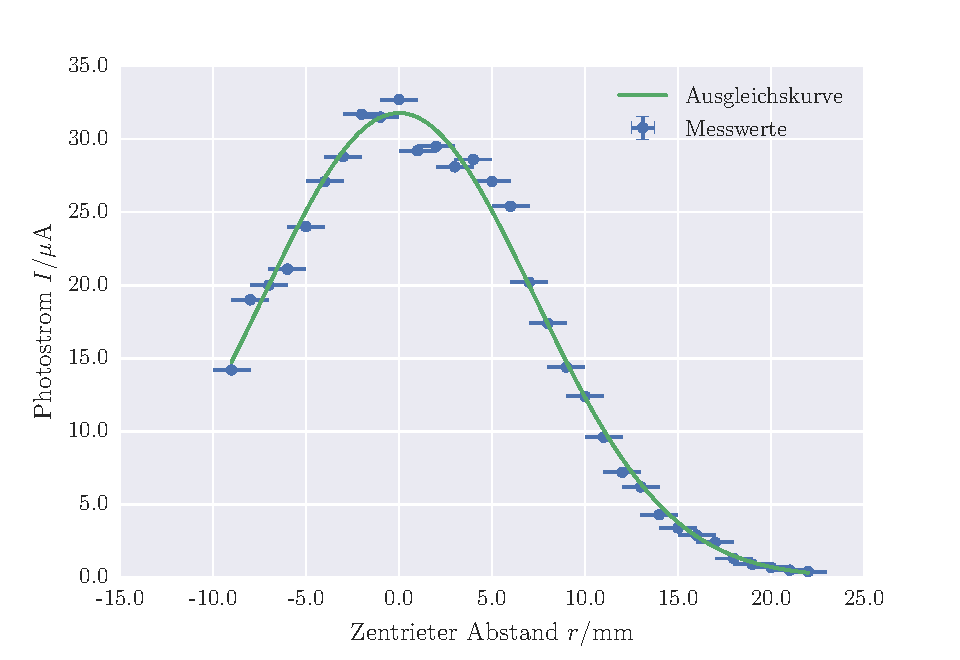
\includegraphics[scale=0.8]{../Grafiken/TEM_00.pdf}
 \caption{Grafische Darstellung des Photostroms in Abhängigkeit des Abstands zur optischen Achse.\label{fig:tem_00}}
 \end{figure} 
	\FloatBarrier	
    Für die Regressionsparameter, Maximalintensität $I_0$ und Stahlbreite $\omega$ ergaben sich 
    dabei die folgenden Werte:
    %Maximalintensität I_0  3.17836425029e-05 +/- 3.51838588946e-08
    %Strahlbreite w         0.0145329570585 +/- 2.21455314836e-05
    \begin{empheq}{align*}
	    I_0 &= \SI{31.78(4)}{\micro\ampere},\\
	    \omega &= \SI{1.453(2)}{\milli\meter}.
    \end{empheq}

	
\subsection[Intensitätverteilung der $\mathrm{TEM_{10}}$]{Intensitätverteilung der $\mathbf{TEM_{10}}$}\label{sec:TEM10}
	Wie schon bei der vorherigen Messung, wurde auch bei der Vermessung der ersten transversalen Mode der Strom 
	an Photodiode in Abhängigkeit des Abstands von der optischen Achse gemessen.
	Die Werte dieser Messung befinden sich in \cref{tab:TEM10}. 
	\begin{table}[!h]
	\centering
	\begin{tabular}{cccc}
		\toprule
		Abstand & Photostrom & Abstand & Photostrom\\
		$r$ [\si{m}] & $I$ [\si{\micro\ampere}] & $x$ [\si{m}] & $I$ [\si{\micro\ampere}]\\
\midrule
		\num{-0.009(1)} & \num{2.7(1)} & \num{0.007(1)} & \num{2.4(1)}\\
		\num{-0.008(1)} & \num{2.5(1)} & \num{0.008(1)} & \num{2.5(1)}\\
		\num{-0.007(1)} & \num{1.9(1)} & \num{0.009(1)} & \num{2.8(1)}\\
		\num{-0.006(1)} & \num{1.7(1)} & \num{0.010(1)} & \num{3.3(1)}\\
		\num{-0.005(1)} & \num{1.5(1)} & \num{0.011(1)} & \num{2.2(1)}\\
		\num{-0.004(1)} & \num{1.2(1)} & \num{0.012(1)} & \num{1.7(1)}\\
		\num{-0.003(1)} & \num{0.8(1)} & \num{0.013(1)} & \num{1.6(1)}\\
		\num{-0.002(1)} & \num{0.3(1)} & \num{0.014(1)} & \num{1.5(1)}\\
		\num{-0.001(1)} & \num{0.2(1)} & \num{0.015(1)} & \num{1.2(1)}\\
		\num{0.000(1)} & \num{0.1(1)} & \num{0.016(1)} & \num{0.9(1)}\\
		\num{0.001(1)} & \num{0.1(1)} & \num{0.017(1)} & \num{0.8(1)}\\
		\num{0.002(1)} & \num{0.3(1)} & \num{0.018(1)} & \num{0.6(1)}\\
		\num{0.003(1)} & \num{0.4(1)} & \num{0.019(1)} & \num{0.5(1)}\\
		\num{0.004(1)} & \num{1.0(1)} & \num{0.020(1)} & \num{0.4(1)}\\
		\num{0.005(1)} & \num{1.7(1)} & \num{0.021(1)} & \num{0.2(1)}\\
		\num{0.006(1)} & \num{2.0(1)} & \num{0.022(1)} & \num{0.1(1)}\\
		\bottomrule
	\end{tabular}
	\caption{Messwerte des Photostroms in Abhaengigkeit des horizontalen Abstands zur optischen Achse. \label{tab:TEM10}}
\end{table}

	\FloatBarrier
	Die grafische Darstellung dieser Daten ist zusammen mit einer Regressionskurve der Form \eqref{eq:tem10}
	in \cref{fig:tem_10} aufgetragen.
	\begin{figure}[!h]
 \centering
 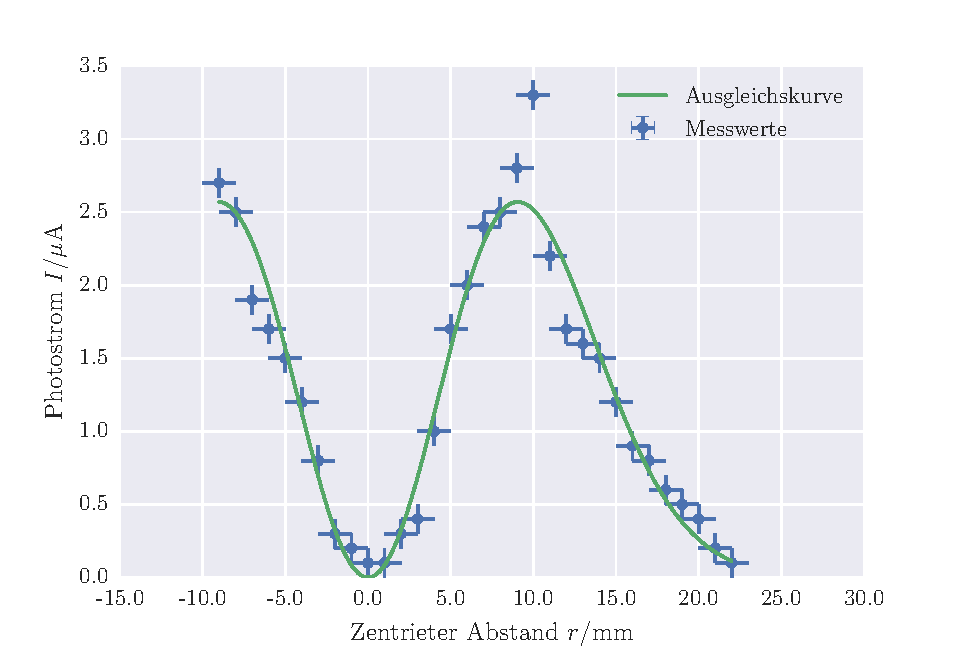
\includegraphics[scale=0.8]{../Grafiken/TEM_10.pdf}
 \caption{Grafische Darstellung der Messwerte des Photostroms in Abhängigkeit des Abstands zur optischen Achse.\label{fig:tem_10}}
 \end{figure} 
	\FloatBarrier
	Hierbei ergaben sich die Regressionsparameter:
	%Maximalintensität I_0  1.74633255993e-06 +/- 1.97895844321e-08
	%Strahlbreite w         -0.01281502869 +/- 0.000101158988474
	\begin{empheq}{align*}
		 I_0 &= \SI{1.75(2)}{\micro\ampere},\\
		 \omega &= \SI{-1.282(1)}{\milli\meter}.
	\end{empheq}
\subsection{Polarisation des Laserlichts}\label{sec:Polarisation}
	Für die Bestimmung der Polarisation des Laserlichts wurde der Strom der Photodiode und somit
	die Intensität der $\mathrm{TEM}_{00}$ in Abhängigkeit des Polarisatorwinkels $\phi$ gemessen. Die dabei aufgenommenen
	Messwerte befinden sich in \cref{tab:Polarisation}. 
	\begin{table}[!h]
	\centering
	%\begin{adjustbox}{height=2.5cm}
	\begin{tabular}{cccc}
		\toprule
		Polarisatorwinkel & Photostrom & Polarisatorwinkel & Photostrom\\
		$\phi$/\si{rad} & $I$/\si{\micro\ampere} & $\phi$/\si{rad} & $I$/\si{\micro\ampere}\\
\midrule
		\num{0.00(2)} & \num{6.7(1)} & \num{3.14(2)} & \num{6.1(1)}\\
		\num{0.35(2)} & \num{11.7(1)} & \num{3.49(2)} & \num{12.3(1)}\\
		\num{0.70(2)} & \num{14.9(1)} & \num{3.84(2)} & \num{16.9(1)}\\
		\num{1.05(2)} & \num{13.3(1)} & \num{4.19(2)} & \num{16.2(1)}\\
		\num{1.40(2)} & \num{11.1(1)} & \num{4.54(2)} & \num{10.3(1)}\\
		\num{1.75(2)} & \num{6.8(1)} & \num{4.89(2)} & \num{7.1(1)}\\
		\num{2.09(2)} & \num{2.1(1)} & \num{5.24(2)} & \num{1.8(1)}\\
		\num{2.44(2)} & \num{0.1(1)} & \num{5.59(2)} & \num{0.1(1)}\\
		\num{2.79(2)} & \num{1.8(1)} & \num{5.93(2)} & \num{2.0(1)}\\
		\bottomrule
	\end{tabular}
	%\end{adjustbox}
	\caption{Messwerte des Photostroms in Abhängigkeit des Polarisationswinkels. \label{tab:Polarisation}}
\end{table}

	\FloatBarrier
	Durch Auftragen der Messwerte ergab sich der in \cref{fig:polarisation} gezeigte Grafik.
	Eine Regressionskurve der Form von \eqref{eq:polarisation} wurde zu den Messwerten erzeugt und
	ebenfalls in \cref{fig:polarisation} eingetragen.
	\begin{figure}[!h]
 \centering
 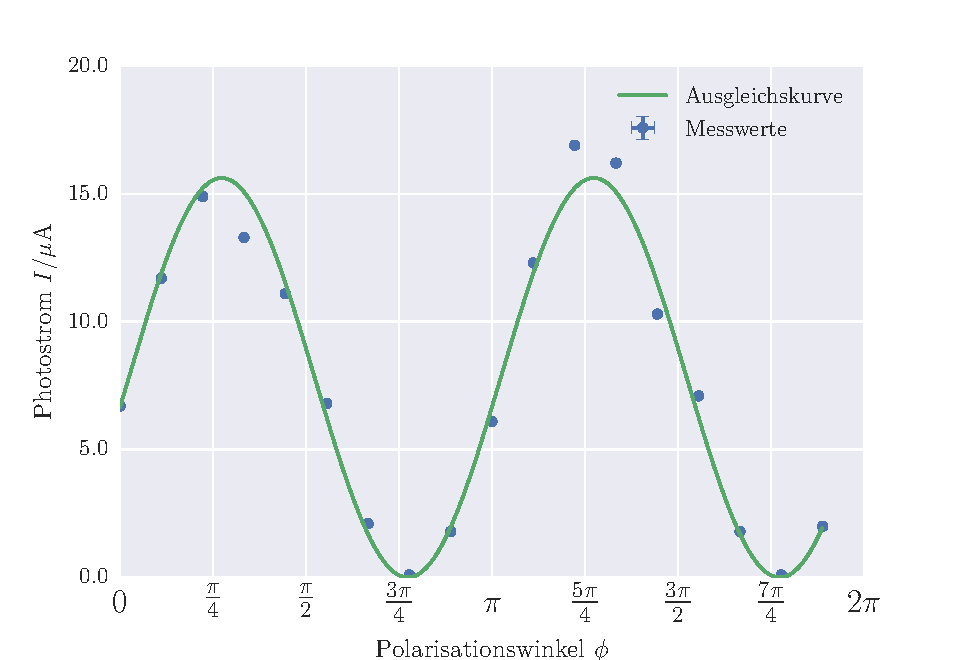
\includegraphics[scale=0.75]{../Grafiken/Polarisation.pdf}
 \caption{Grafische Darstellung der aufgenommenen Messwerte des Photostroms in Abhängigkeit des, am Polarisator eingestellten, Winkels.\label{fig:polarisation}}
 \end{figure} 
	\FloatBarrier
	Für die Maximalintensität $I_0$ und den Phasenwinkel $\phi_0$ ergab die Regression die Werte
	
	%Maximalintensität I_0  1.56217702188e-05 +/- 3.84900177443e-08
	%Phase phi_0            2.42987521953 +/- 0.00213377505421
	
	\begin{empheq}{align*}
		I_0 &= \SI{15.62(4)}{\micro\ampere},\\
		\phi_0 &= \SI{2.430(2)}{rad},\\
			   &= \SI{139.2(1)}{\degree}.
	\end{empheq}
	
%	Aus dem Phasenwinkel $\phi_0$ konnte der Polarisationswinkel des Laserlichts, unter Zuhilfenahme von \eqref{eq:polarisation_laser}, zu
%	\begin{empheq}{align*}
%			\phi_{\mathrm{p}} &= \SI{0.859(2)}{rad}\\
%							  &= \SI{49.2(1)}{\degree}
%	\end{empheq}
%	berechnet werden.	

\subsection{Wellenlänge des Laserlichts}\label{sec:Wellenlaenge}
	Die zur Bestimmung der Wellenlänge aufgenommenen Daten befinden sich in \cref{tab:Wellenlaengen}. Für Umrechnung
	der gemessenen Abstände zum Hauptmaximum $d$ in die nötigen Beugungswinkel $\theta$, mittels \eqref{eq:gitter_winkel}, 
	wurde noch der Abstand vom Gitter zum Hauptmaximum $l = \SI{1.085(1)}{m}$ gemessen. Die in \cref{tab:Wellenlaengen}  eingetragenen Wellenlängen 
	berechneten sich aus den Winkel und der Gitterkonstante des verwendeten Gitters, $g = \SI{0.01}{mm}$, nach \eqref{eq:gitter}.
	\begin{table}[!h]
	\centering
	\begin{tabular}{ccc}
		\toprule
		Abstand & Winkel & Wellenlaenge\\
		$d$ [\si{m}] & $\theta$ [\si{rad}] & $\lambda$ [\si{\micro\meter}]\\
\midrule
		\num{0.070(1)} & \num{0.0644(9)} & \num{0.644(9)}\\
		\num{0.140(1)} & \num{0.1283(9)} & \num{0.640(5)}\\
		\num{0.210(1)} & \num{0.1912(9)} & \num{0.633(3)}\\
		\num{0.284(1)} & \num{0.2560(9)} & \num{0.633(2)}\\
		\num{0.364(1)} & \num{0.3237(9)} & \num{0.636(2)}\\
		\bottomrule
	\end{tabular}
	\caption{Messwerte der Abstaende zwischen den Maxima dem Hauptmaximum und die resultierenden Winkel und Wellenlaengen. \label{tab:Wellenlaengen}}
\end{table}

	\FloatBarrier
	Als Mittelwert der Wellenlänge ergab sich in dieser Messung:
	\begin{empheq}{equation*}
		\mean{\lambda} = \SI[parse-numbers=false]{637 \pm 2(sys) \pm 2(stat)}{nm}
	\end{empheq} 
	Dabei berechnet sich der systematische Fehler aus den Fehlern der einzelnen Messungen durch gaußsche Fehlerfortpflanzung
	\eqref{eq:Fehlerforpflanzung}, wohingegen der statistische Fehler die Standardabweichung vom Mittelwert nach \eqref{eq:Mittelwert_Std}
	darstellt.
	
	
\subsection{Prüfung der Stabilitätsbedingung}\label{sec:Stabilitaetsbedingung}
	Die für die Überprüfung der Stabilitätsbedingung aufgenommenen Messwerte, für Resonatorlänge und Photostrom
	sind in \cref{tab:Stabilität} zu finden\footnote{Einer der Messwerte wurde dabei ausgelassen, da dieser im Vergleich zu den anderen Messwerten eine so starke Abweichung nach oben aufwies, dass eine Verwendung keinen Nutzen gehabt hätte}. Der skalierte Photostrom berechnet sich durch Normierung der Messwerte
	mit dem Maximalwert $I_0 = \SI{81(1)}{\micro\ampere}$ und durch Multiplikation mit dem Wert $c = \num{0.1875}$ der Theoriekurve 
	bei der Resonatorlänge $L = \SI{0.65}{\meter}$. Diese Skalierung wurde vorgenommen um die aufgenommenen Messwerte 
	und die, mit diesen in \cref{fig:stabilitaetsbedingung} eingetragene, Theoriekurve vergleichen zu können.
	Neben den Messwerten und der Theoriekurve ist in
	\cref{fig:stabilitaetsbedingung} eine Regressionskurve der Form
	\begin{empheq}{equation}
		g_1g_2(L) = a \cdot L^2 + b \cdot L + c,
	\end{empheq}
	eingetragen. Für die Regressionsparameter $a$,$b$ und $c$ ergaben sich dabei 
	folgende Werte:
	%a  -0.217389075608 +/- 0.0562268753365
	%b  -0.0773822497148 +/- 0.0960797432059
	%c  0.326194436181 +/- 0.0401763378603
	\addtocounter{equation}{-1}
	\begin{subequations}
		\begin{empheq}{align}
			a &= \SI{-0.22(6)}{\per\square\meter},\\
			b &= \SI{-0.1(1)}{\per\meter},\\
			c &= \SI{0.33(4)}{}.
		\end{empheq}
	\end{subequations}

	
	
	\begin{table}[!h]
	\centering
	\begin{tabular}{ccc}
		\toprule
		Resonatorlaenge & Photostrom & Skalierter Photostrom\\
		$L$ [\si{\meter}] & $I$ [\si{\milli\ampere}] & $\frac{I\cdot c}{I_0}$\\
\midrule
		\num{0.65(1)} & \num{0.081(1)} & \num{0.187(2)}\\
		\num{0.70(1)} & \num{0.070(1)} & \num{0.162(2)}\\
		\num{0.75(1)} & \num{0.062(1)} & \num{0.144(2)}\\
		\num{0.80(1)} & \num{0.055(1)} & \num{0.127(2)}\\
		\num{0.85(1)} & \num{0.044(1)} & \num{0.102(2)}\\
		\num{0.95(1)} & \num{0.024(1)} & \num{0.056(2)}\\
		\num{1.00(1)} & \num{0.017(1)} & \num{0.039(2)}\\
		\num{1.05(1)} & \num{0.000(1)} & \num{0.000(2)}\\
		\bottomrule
	\end{tabular}
	\caption{Messwerte des Photostroms und der daraus berechnete, skalierter Photostrom, in Abhaengigkeit der Resonatorlaenge. \label{tab:Stabilitaet}}
\end{table}

	\begin{figure}[!h]
 \centering
 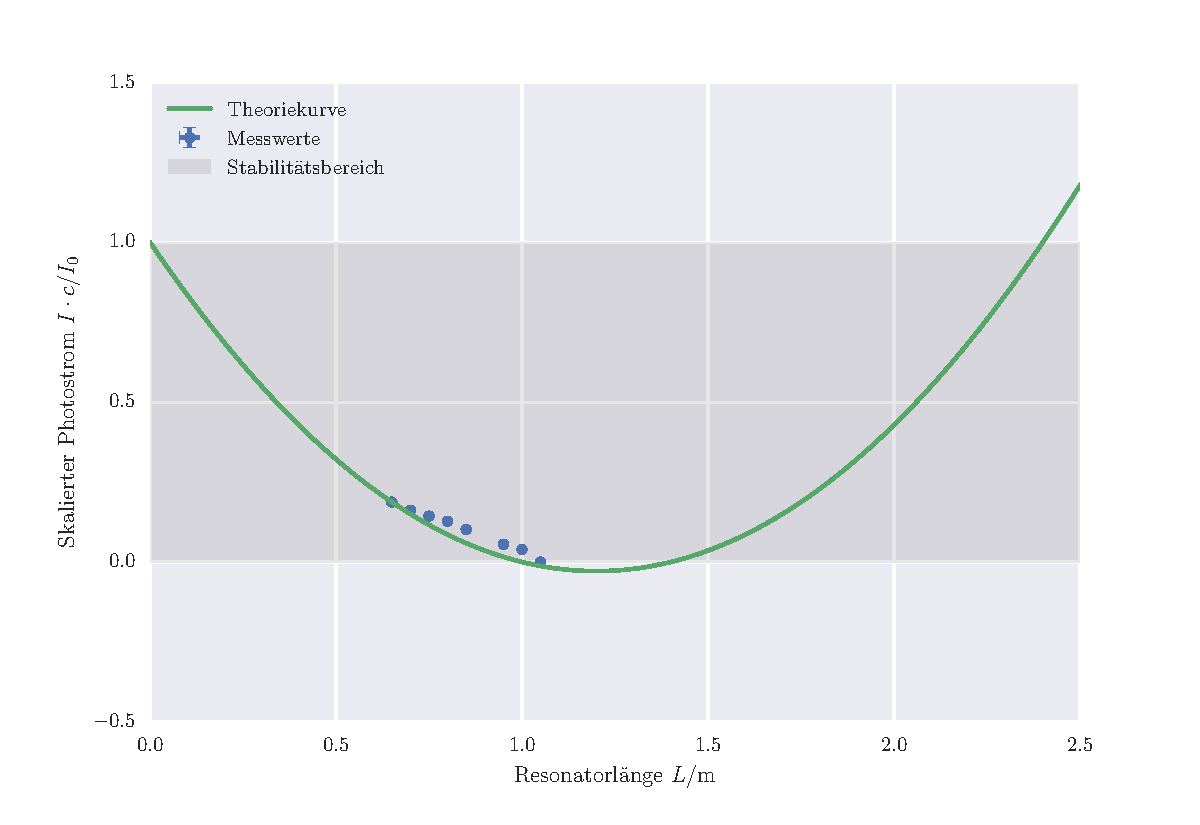
\includegraphics[scale=1]{../Grafiken/Stabilitaetsbedingung.pdf}
 \caption{Grafische Darstellung des skalierten Photostroms in Abhängigkeit der Resonatorlänge.\label{fig:stabilitaetsbedingung}}
 \end{figure} 
	\FloatBarrier